\documentclass{beamer}  
\usepackage{amsmath}
\usepackage{graphicx}
\usepackage{url}
\usepackage{color}

\makeatletter
\def\url@smallurlstyle{%
 \@ifundefined{selectfont}{\def\UrlFont{\sf}}{\def\UrlFont{\footnotesize\ttfamily}}}
\makeatother
\urlstyle{smallurl}

\mode<presentation>
{ \usetheme{Darmstadt} }

\title{Mesh Networking for in Cave Communications\\2025 Update}

\institute{Open SDR}
\author{Philip Balister\inst{1} }
\institute{\inst{1} OpenSDR {\tt\tiny philip@opensdr.com} }

\date{July 10, 2026}
 
\begin{document} 

\begin{frame}
\titlepage
\end{frame}

\section*{Outline}

\begin{frame}
  \tableofcontents
\end{frame}

\section{Background}

\begin{frame}
\frametitle{Open source}

\begin{itemize}
\item I am an Open Source Hippie
\item I know very little about closed source proprietary solutions
\item (and I really don't care)
\item Don't trust your precious cave data to proprietary software!
\item \tiny\url{https://radiolocation.weebly.com/}
\end{itemize}

\end{frame}

\begin{frame}
\frametitle{Why did I do this?}

\begin{itemize}
	\item I've been on the UK Austria Loser Epxedition
	\item In 2025, I took my drone to help prospect
	\item Loser is basically a limestone plateau, with a low scrub pine
	\item I took some photos, then the weather was bad for several days
\end{itemize}

\end{frame}


\begin{frame}
\frametitle{Canonical Loser View}
\begin{center}
\includegraphics[width=4.0in]{../images/Loser.jpg}
\end{center}
\end{frame}

\begin{frame}
\frametitle{Random Drone Photo}
\begin{center}
\includegraphics[width=4.0in]{../images/random-drone.jpg}
\end{center}
\end{frame}

\section{What do you do with random drone photos}

\begin{frame}
\frametitle{Drone photos}

\begin{itemize}
	\item Photos are geotagged
	\item Hard to get context from individual photos
	\item Manually lining up photos is a pain
	\item And the weather was crappy for several days
	\item \tiny\url{https://archive.fosdem.org/2017/schedule/event/geo_drone/}
\end{itemize}
\end{frame}

\begin{frame}
\frametitle{Basics ofPhotogrammetry}

\begin{itemize}
\item Overlapping photos taken from different locations create 3d images
\end{itemize}

\end{frame}


\begin{frame}

\frametitle{Meshtastic Operation}

\begin{itemize}
\item Designed to flood the mesh and assumes multiple routes available
\item When a packet is retransmitted, the hop limit is decremented
\item An node does not retransmit a packet it has heard before
\item A packet is considered acknowledged when the sending node receives it
\item Typical hop limit is set to 3, maximum of 7
\item Nodes check if the channel is busy before transmitting
\item The weaker the received packet is, the sooner a node retransmits it
\end{itemize}

\end{frame}

\begin{frame}
\frametitle{Node Construction}

\begin{center}
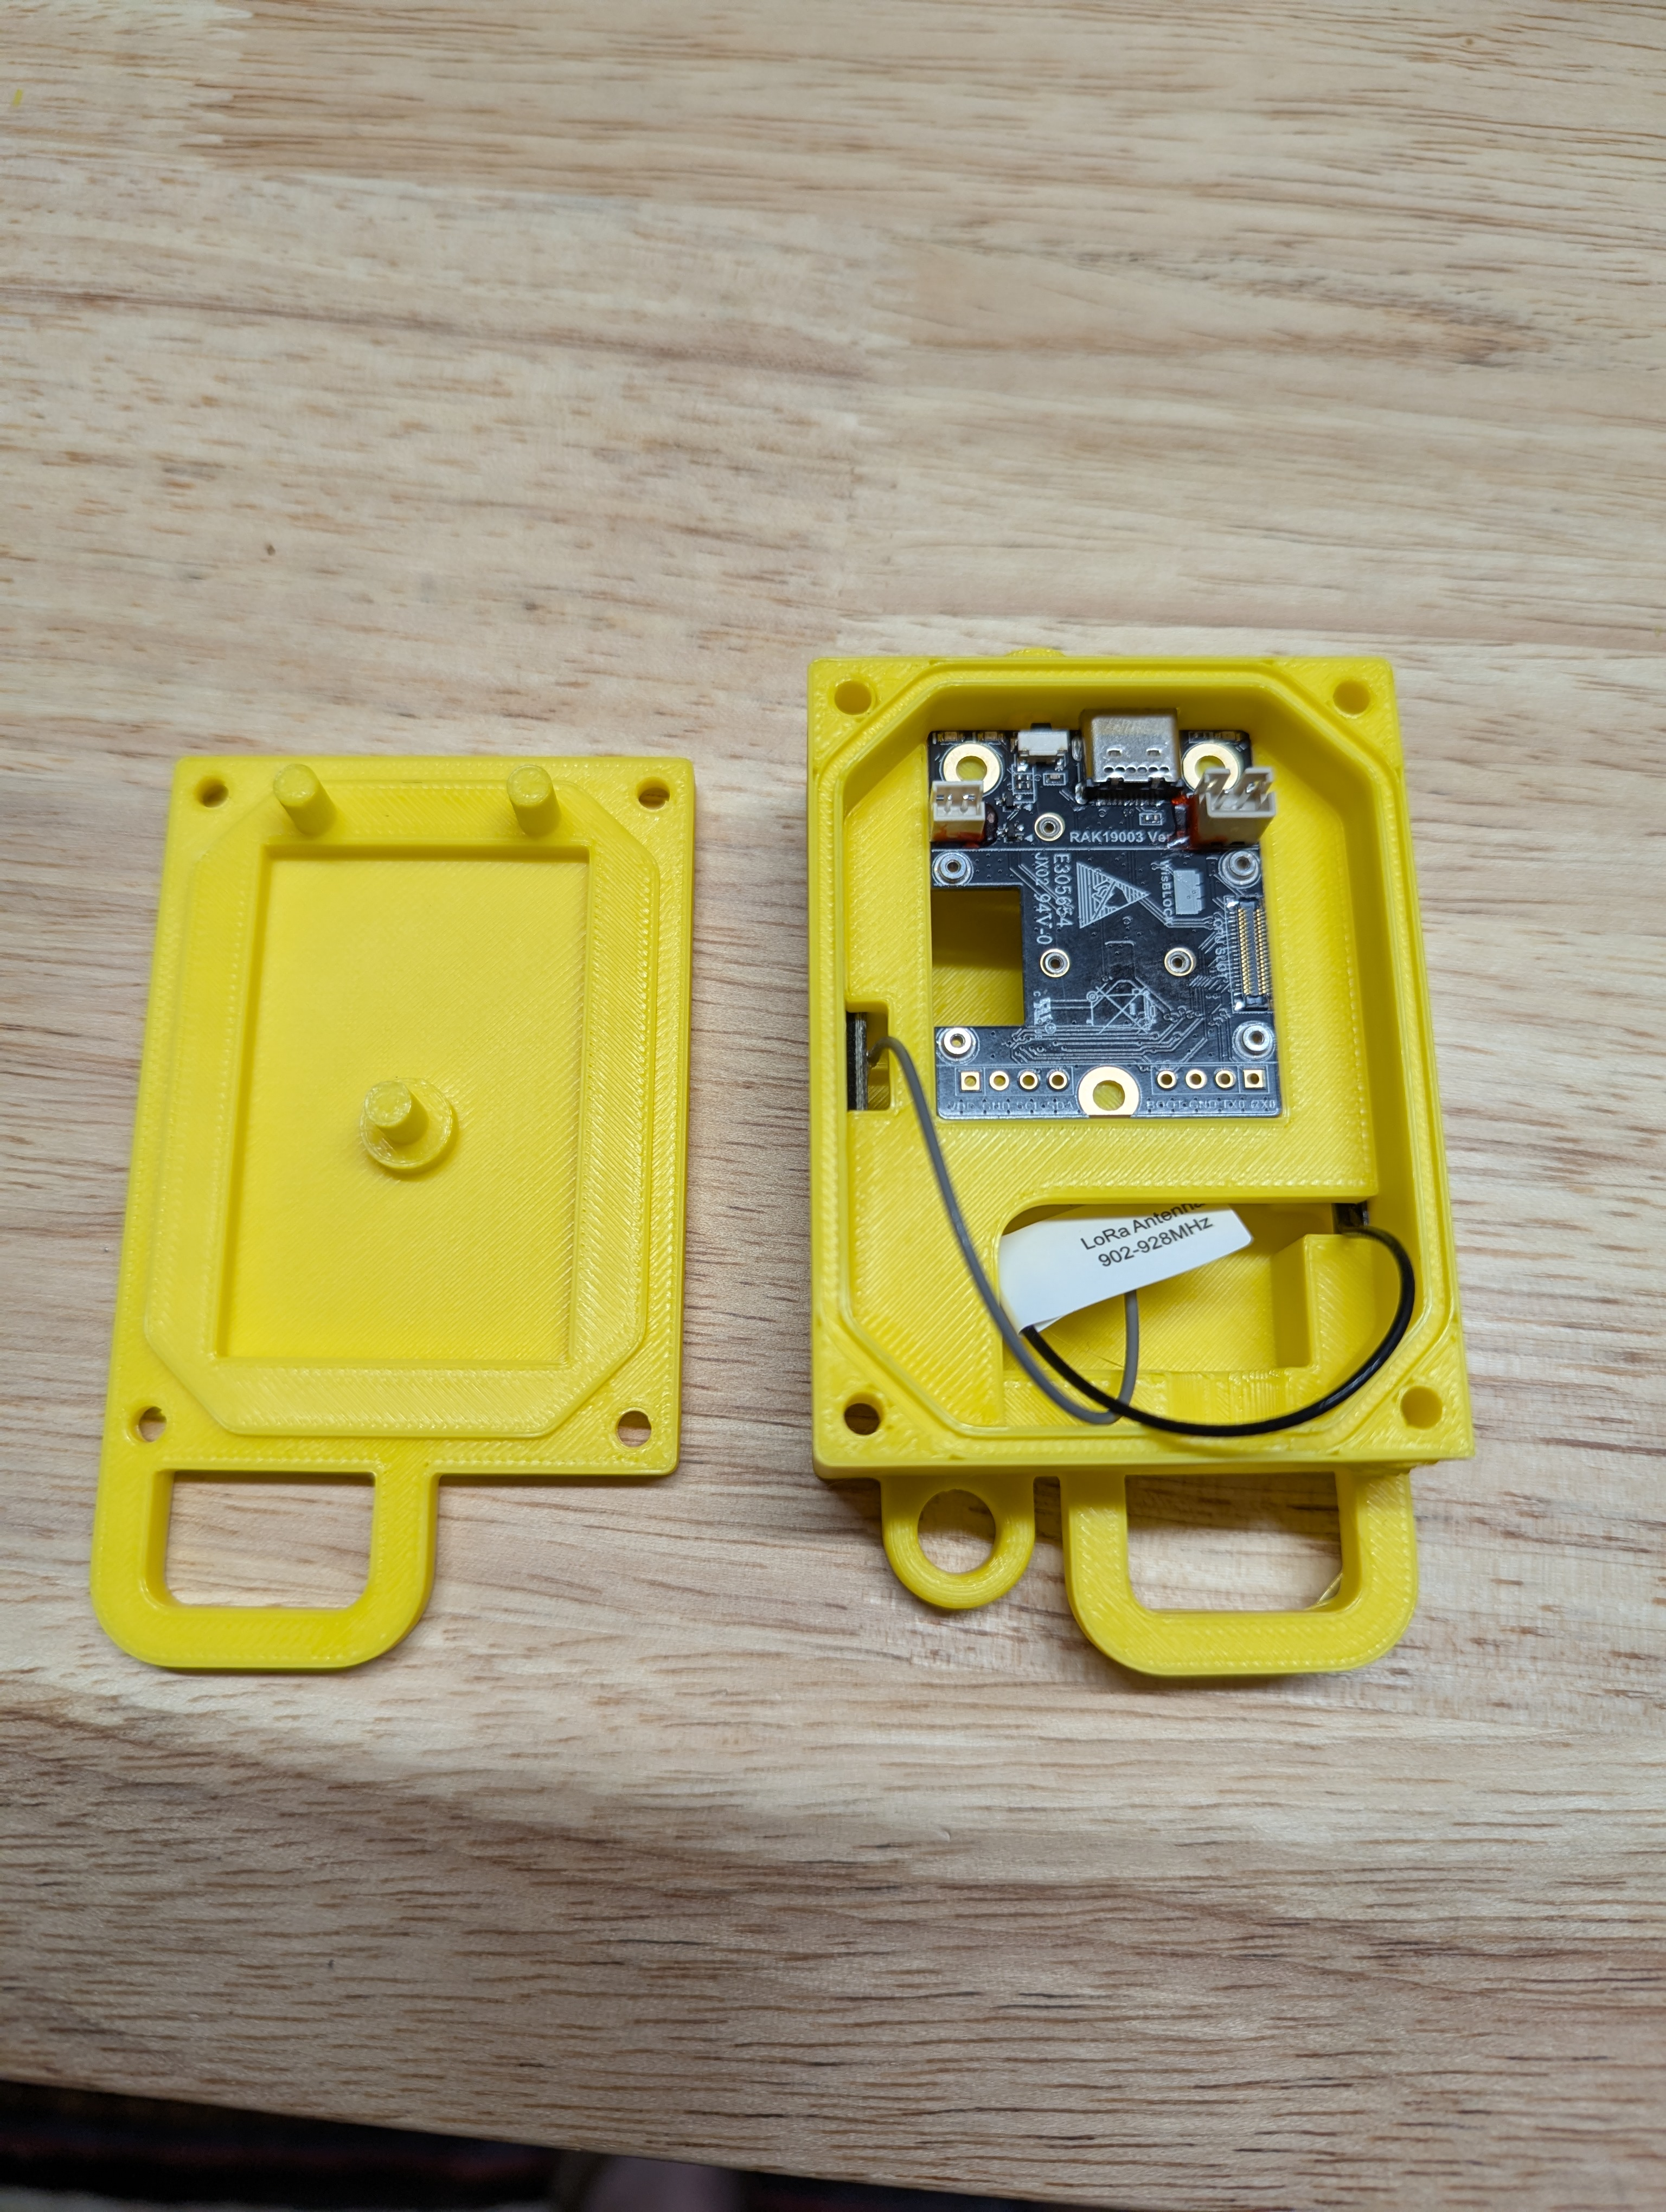
\includegraphics[width=.47\textwidth]{../images/new-case.jpg}\hfill
\end{center}

\end{frame}

\section{In Cave Testing}

\begin{frame}
\frametitle{Nodes In Cave}

\begin{center}
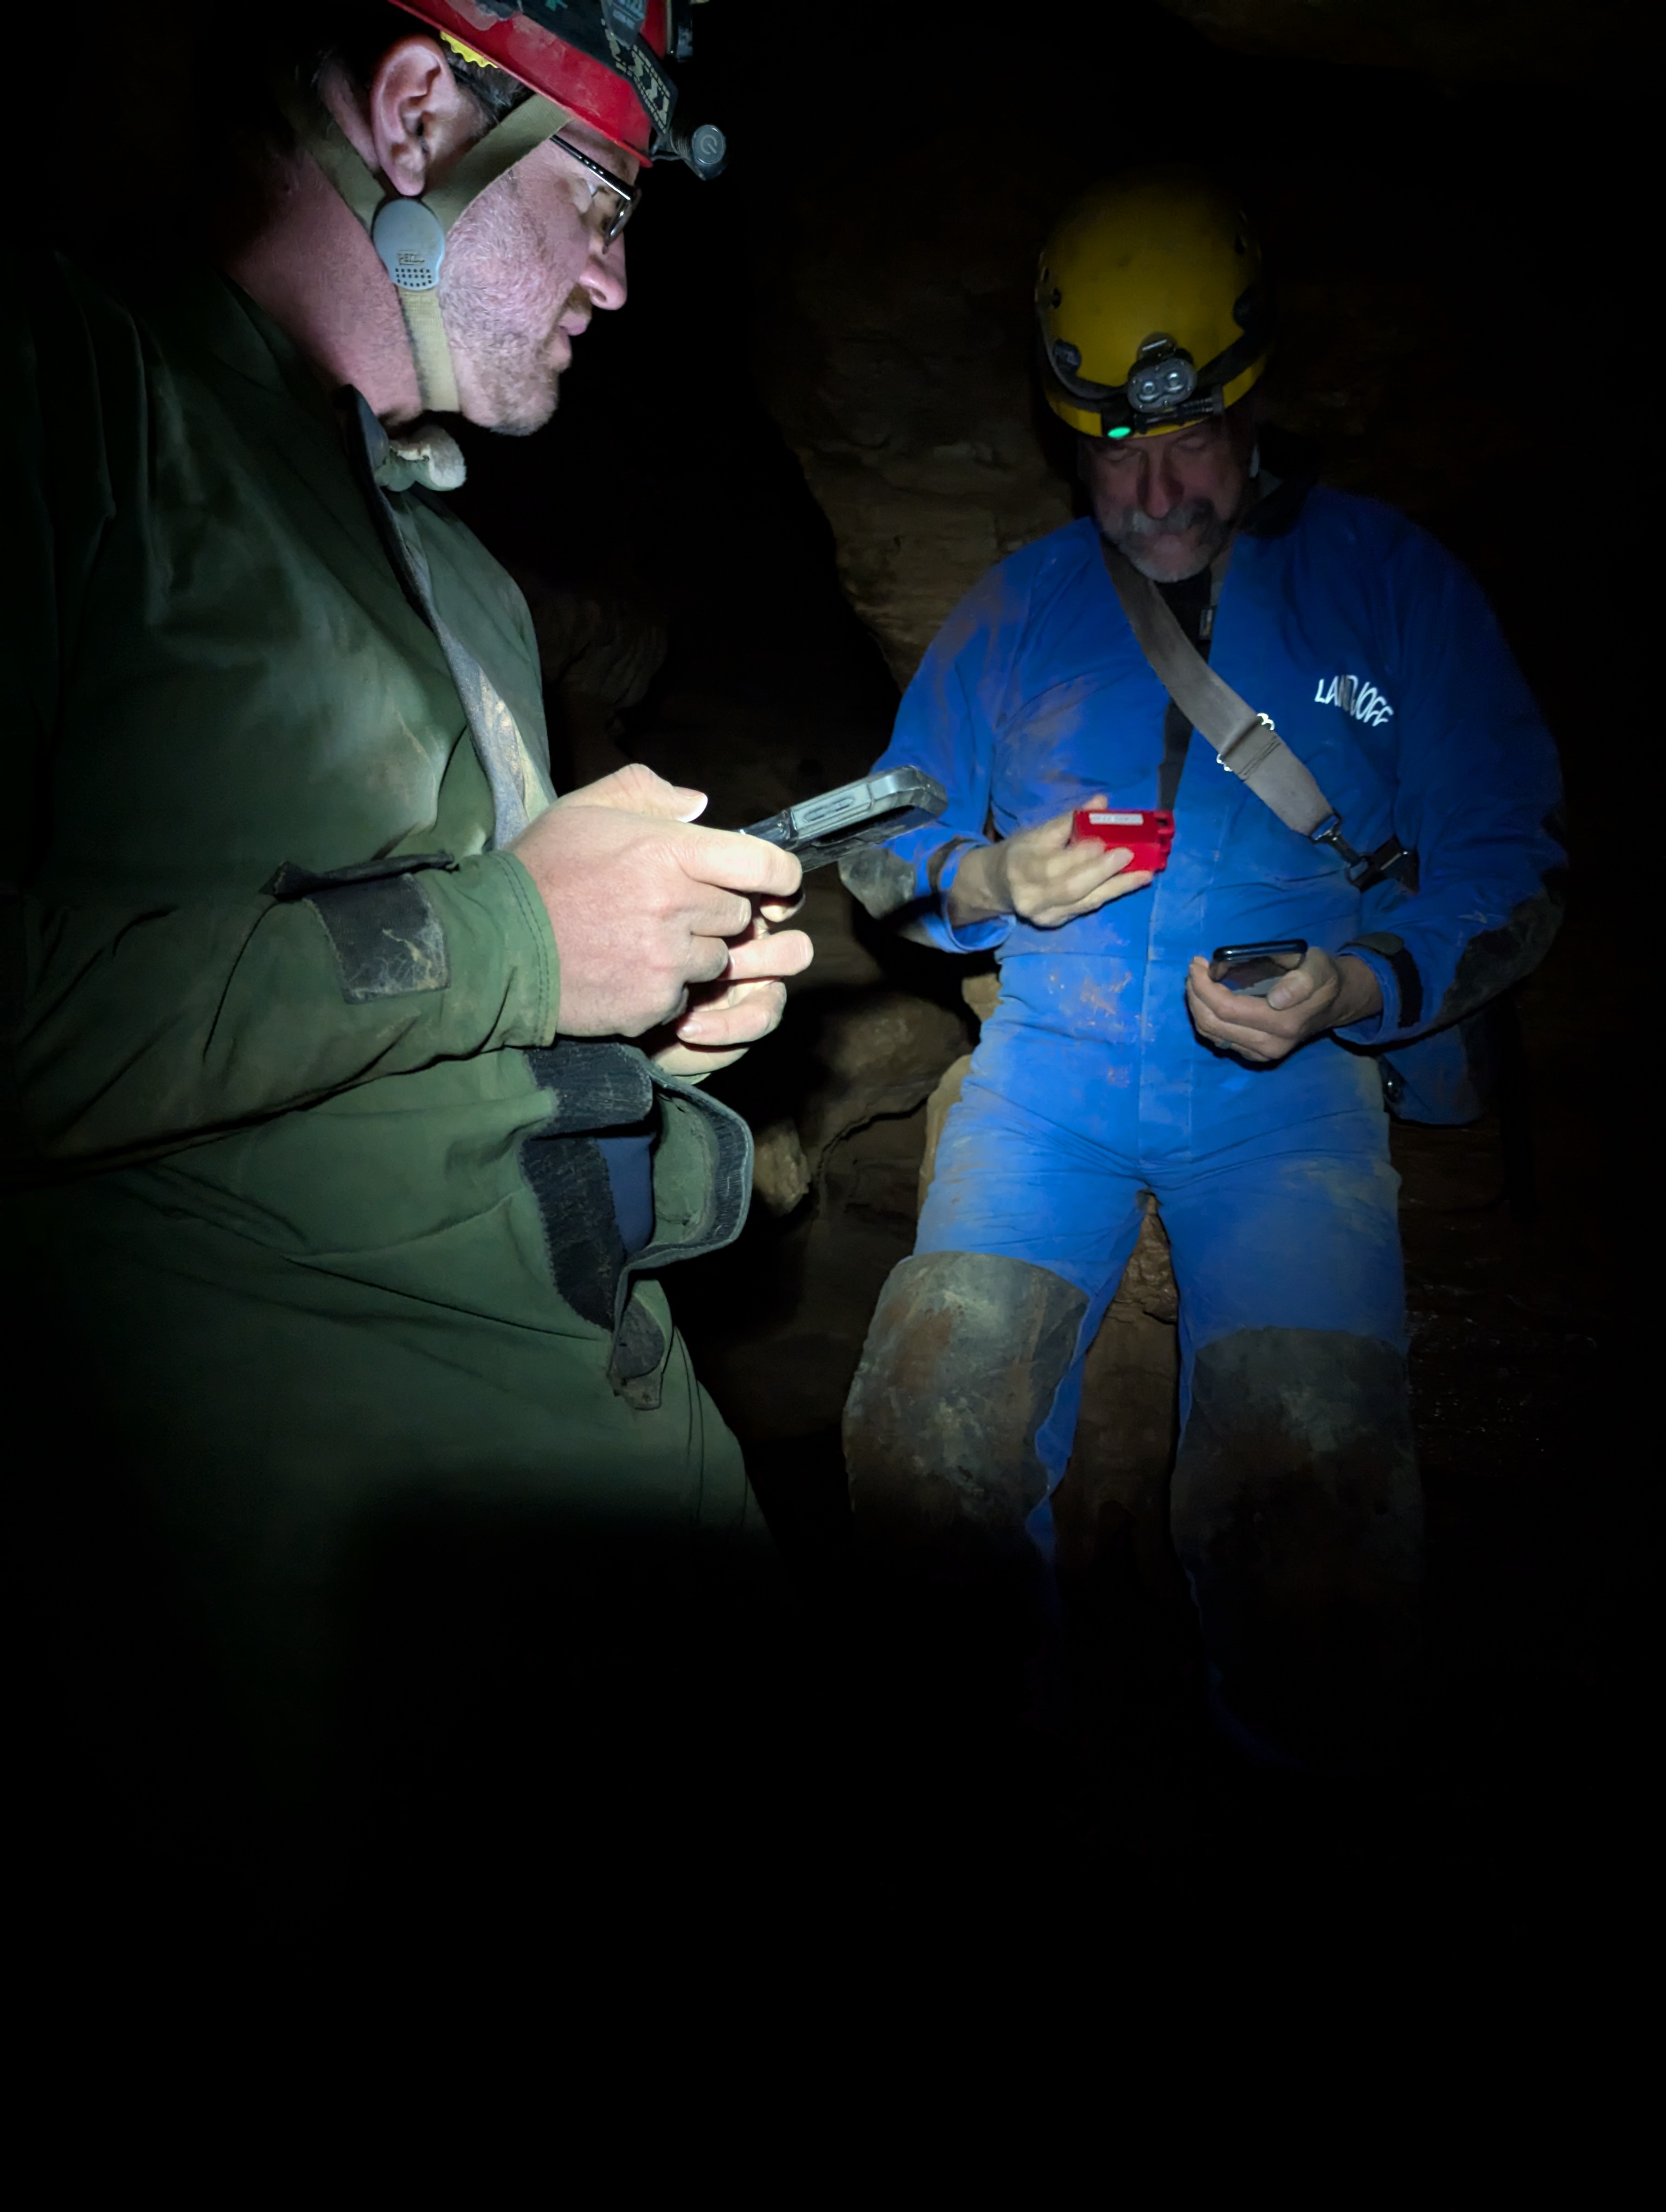
\includegraphics[width=.47\textwidth]{../images/PXL_20250425_162817720.jpg}\hfill
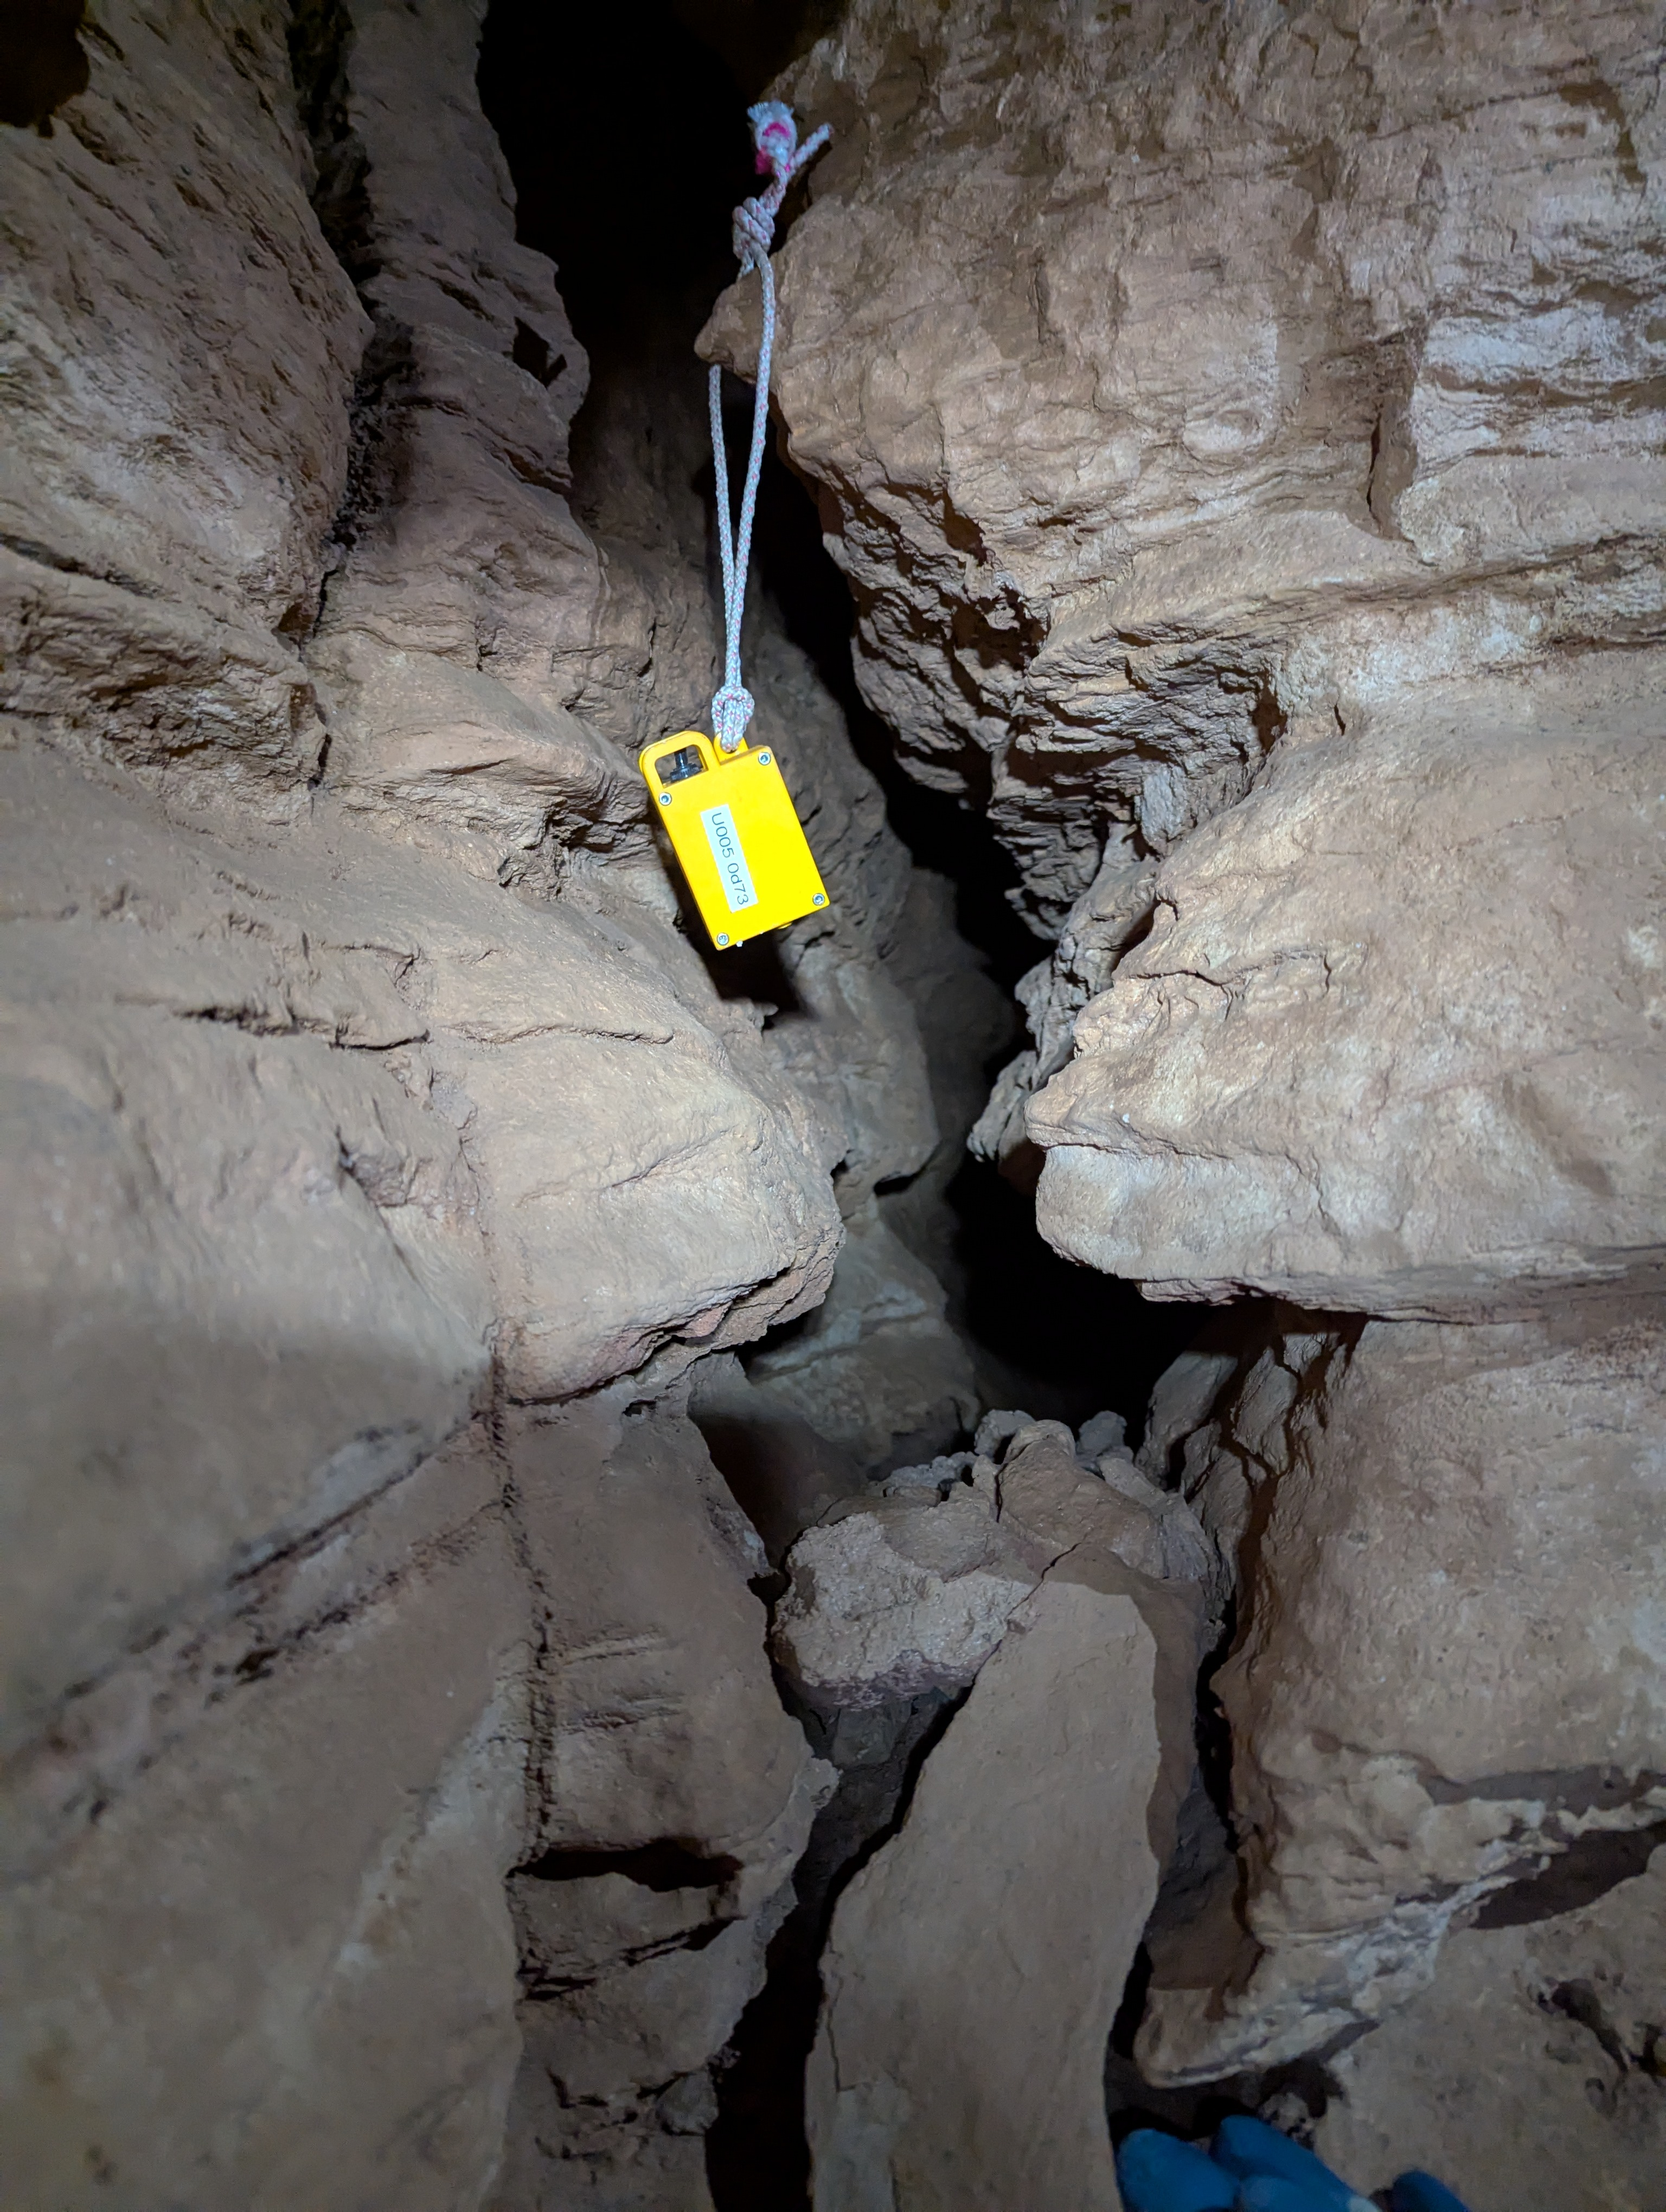
\includegraphics[width=.47\textwidth]{../images/PXL_20250425_165505959.jpg}
\end{center}

\end{frame}

\begin{frame}
\frametitle{More Nodes In Cave}

\begin{center}
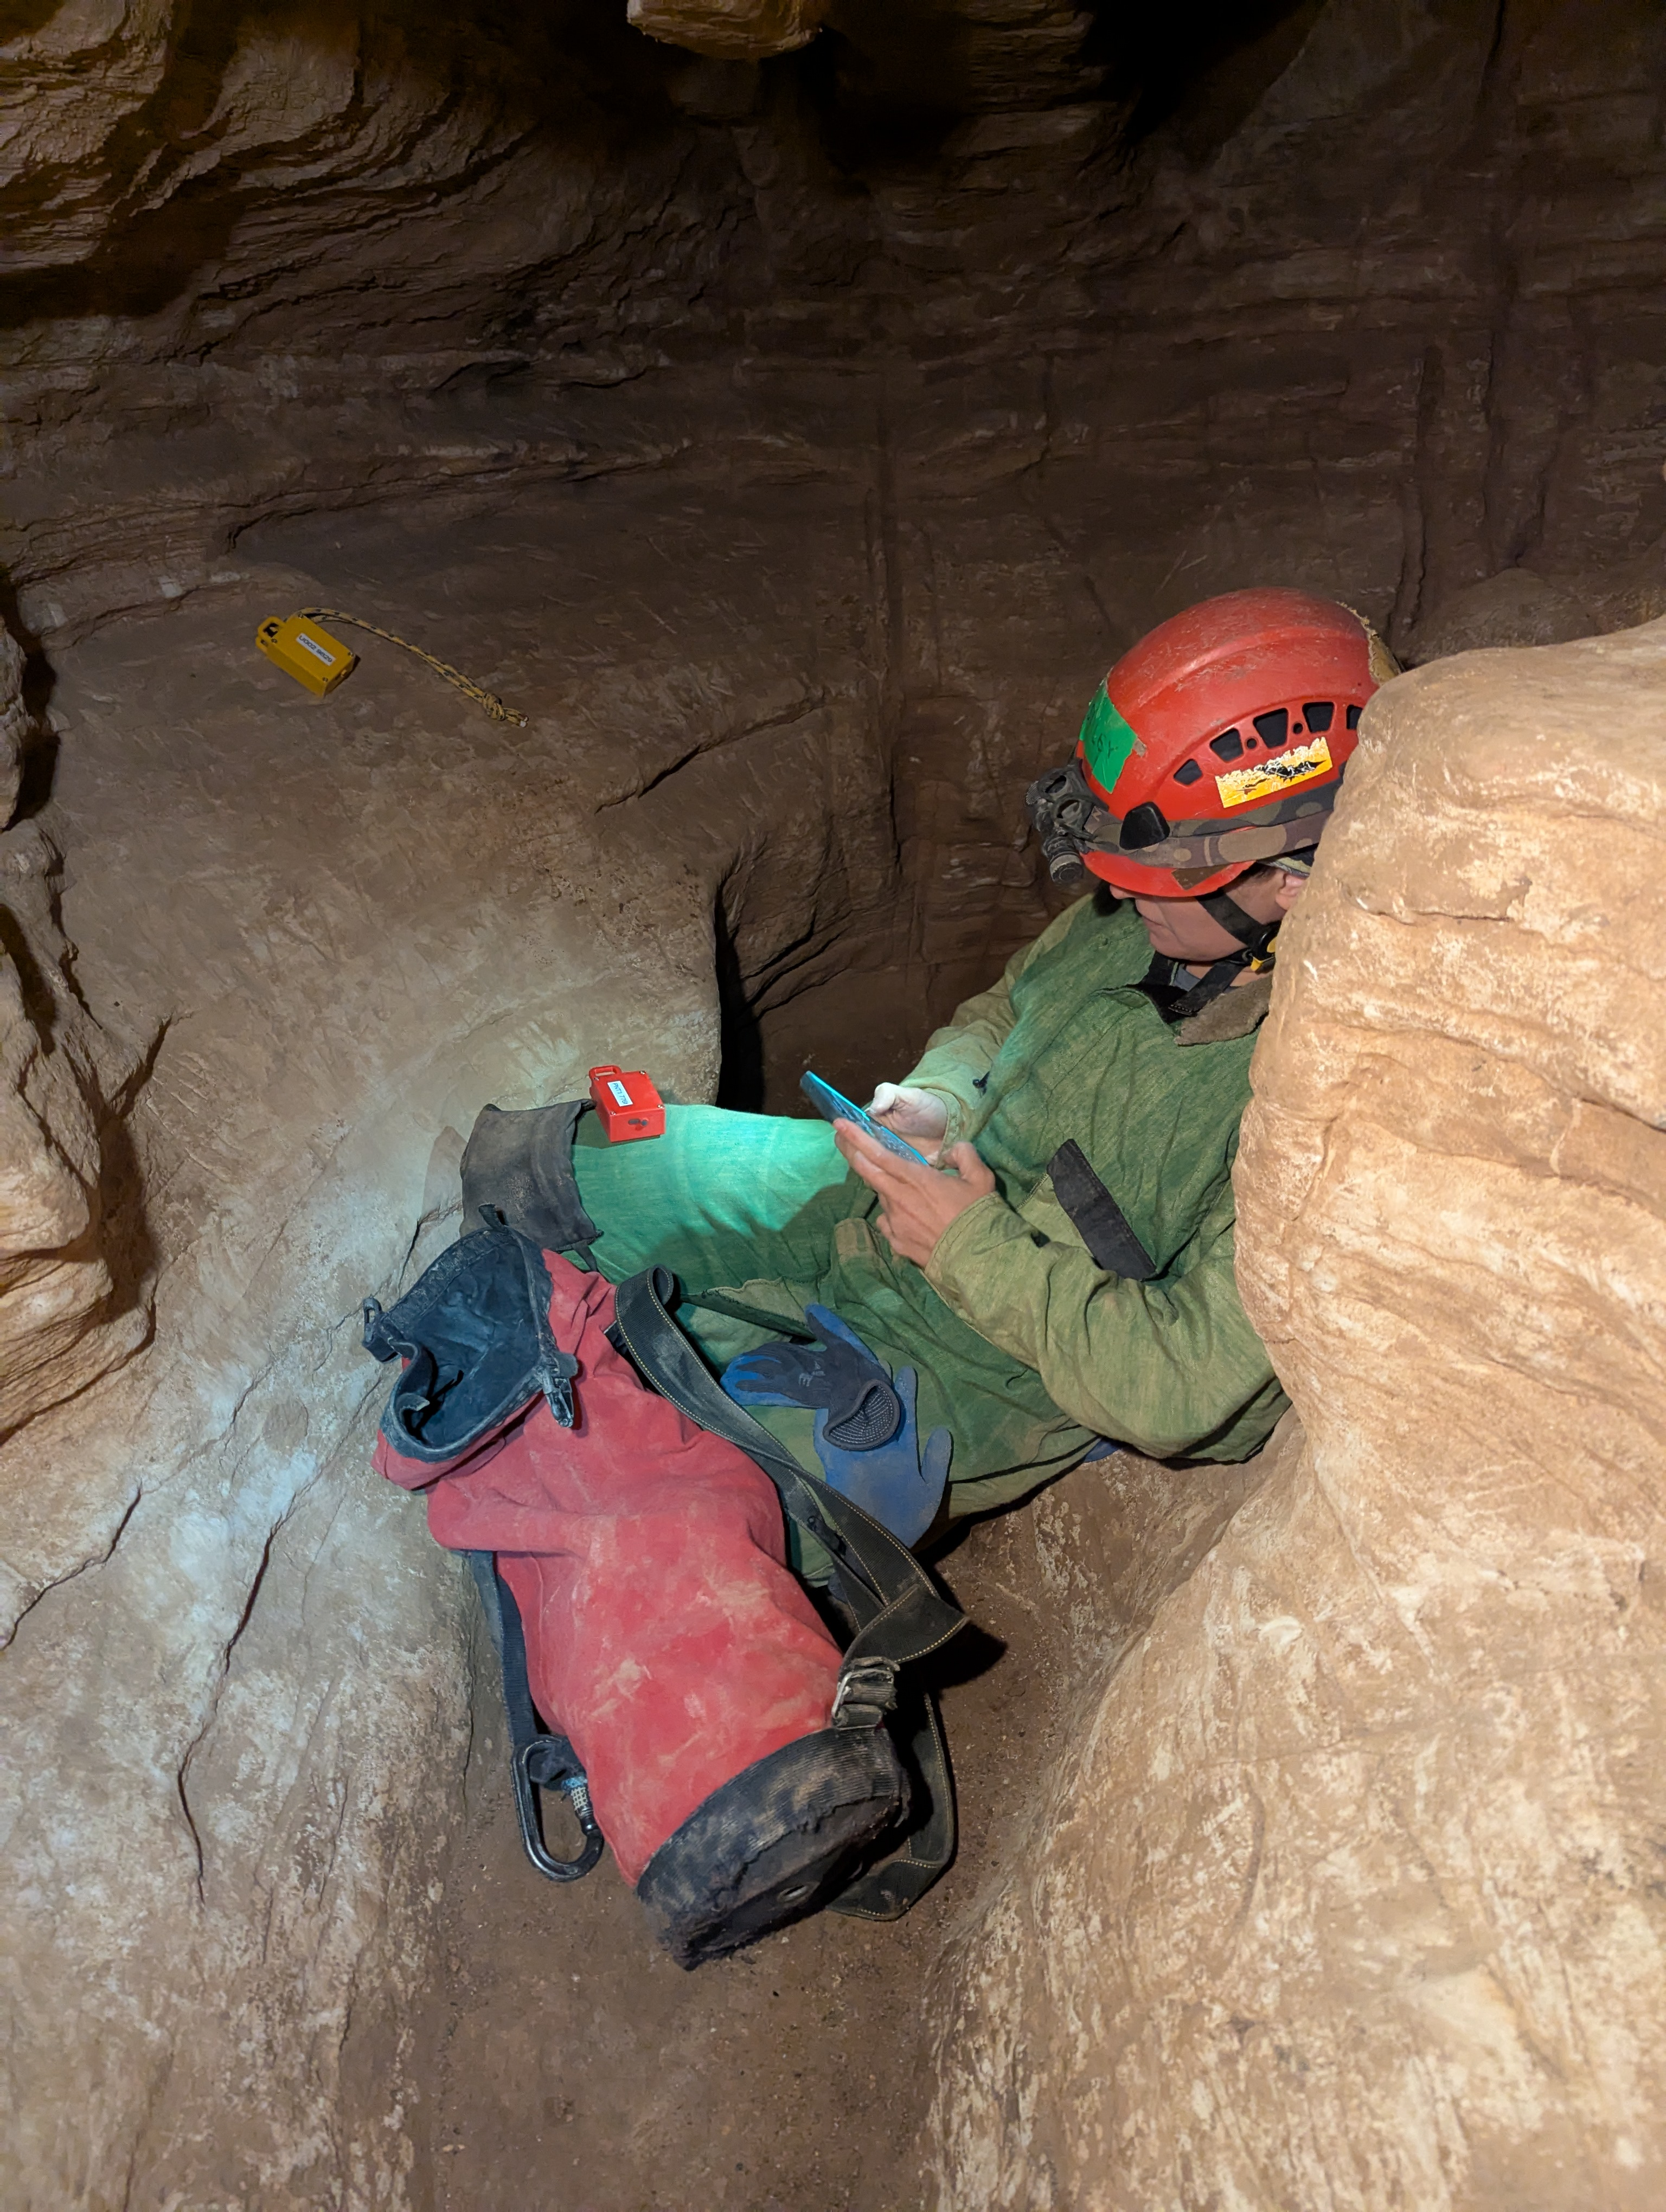
\includegraphics[width=.47\textwidth]{../images/PXL_20250425_170556534.jpg}\hfill
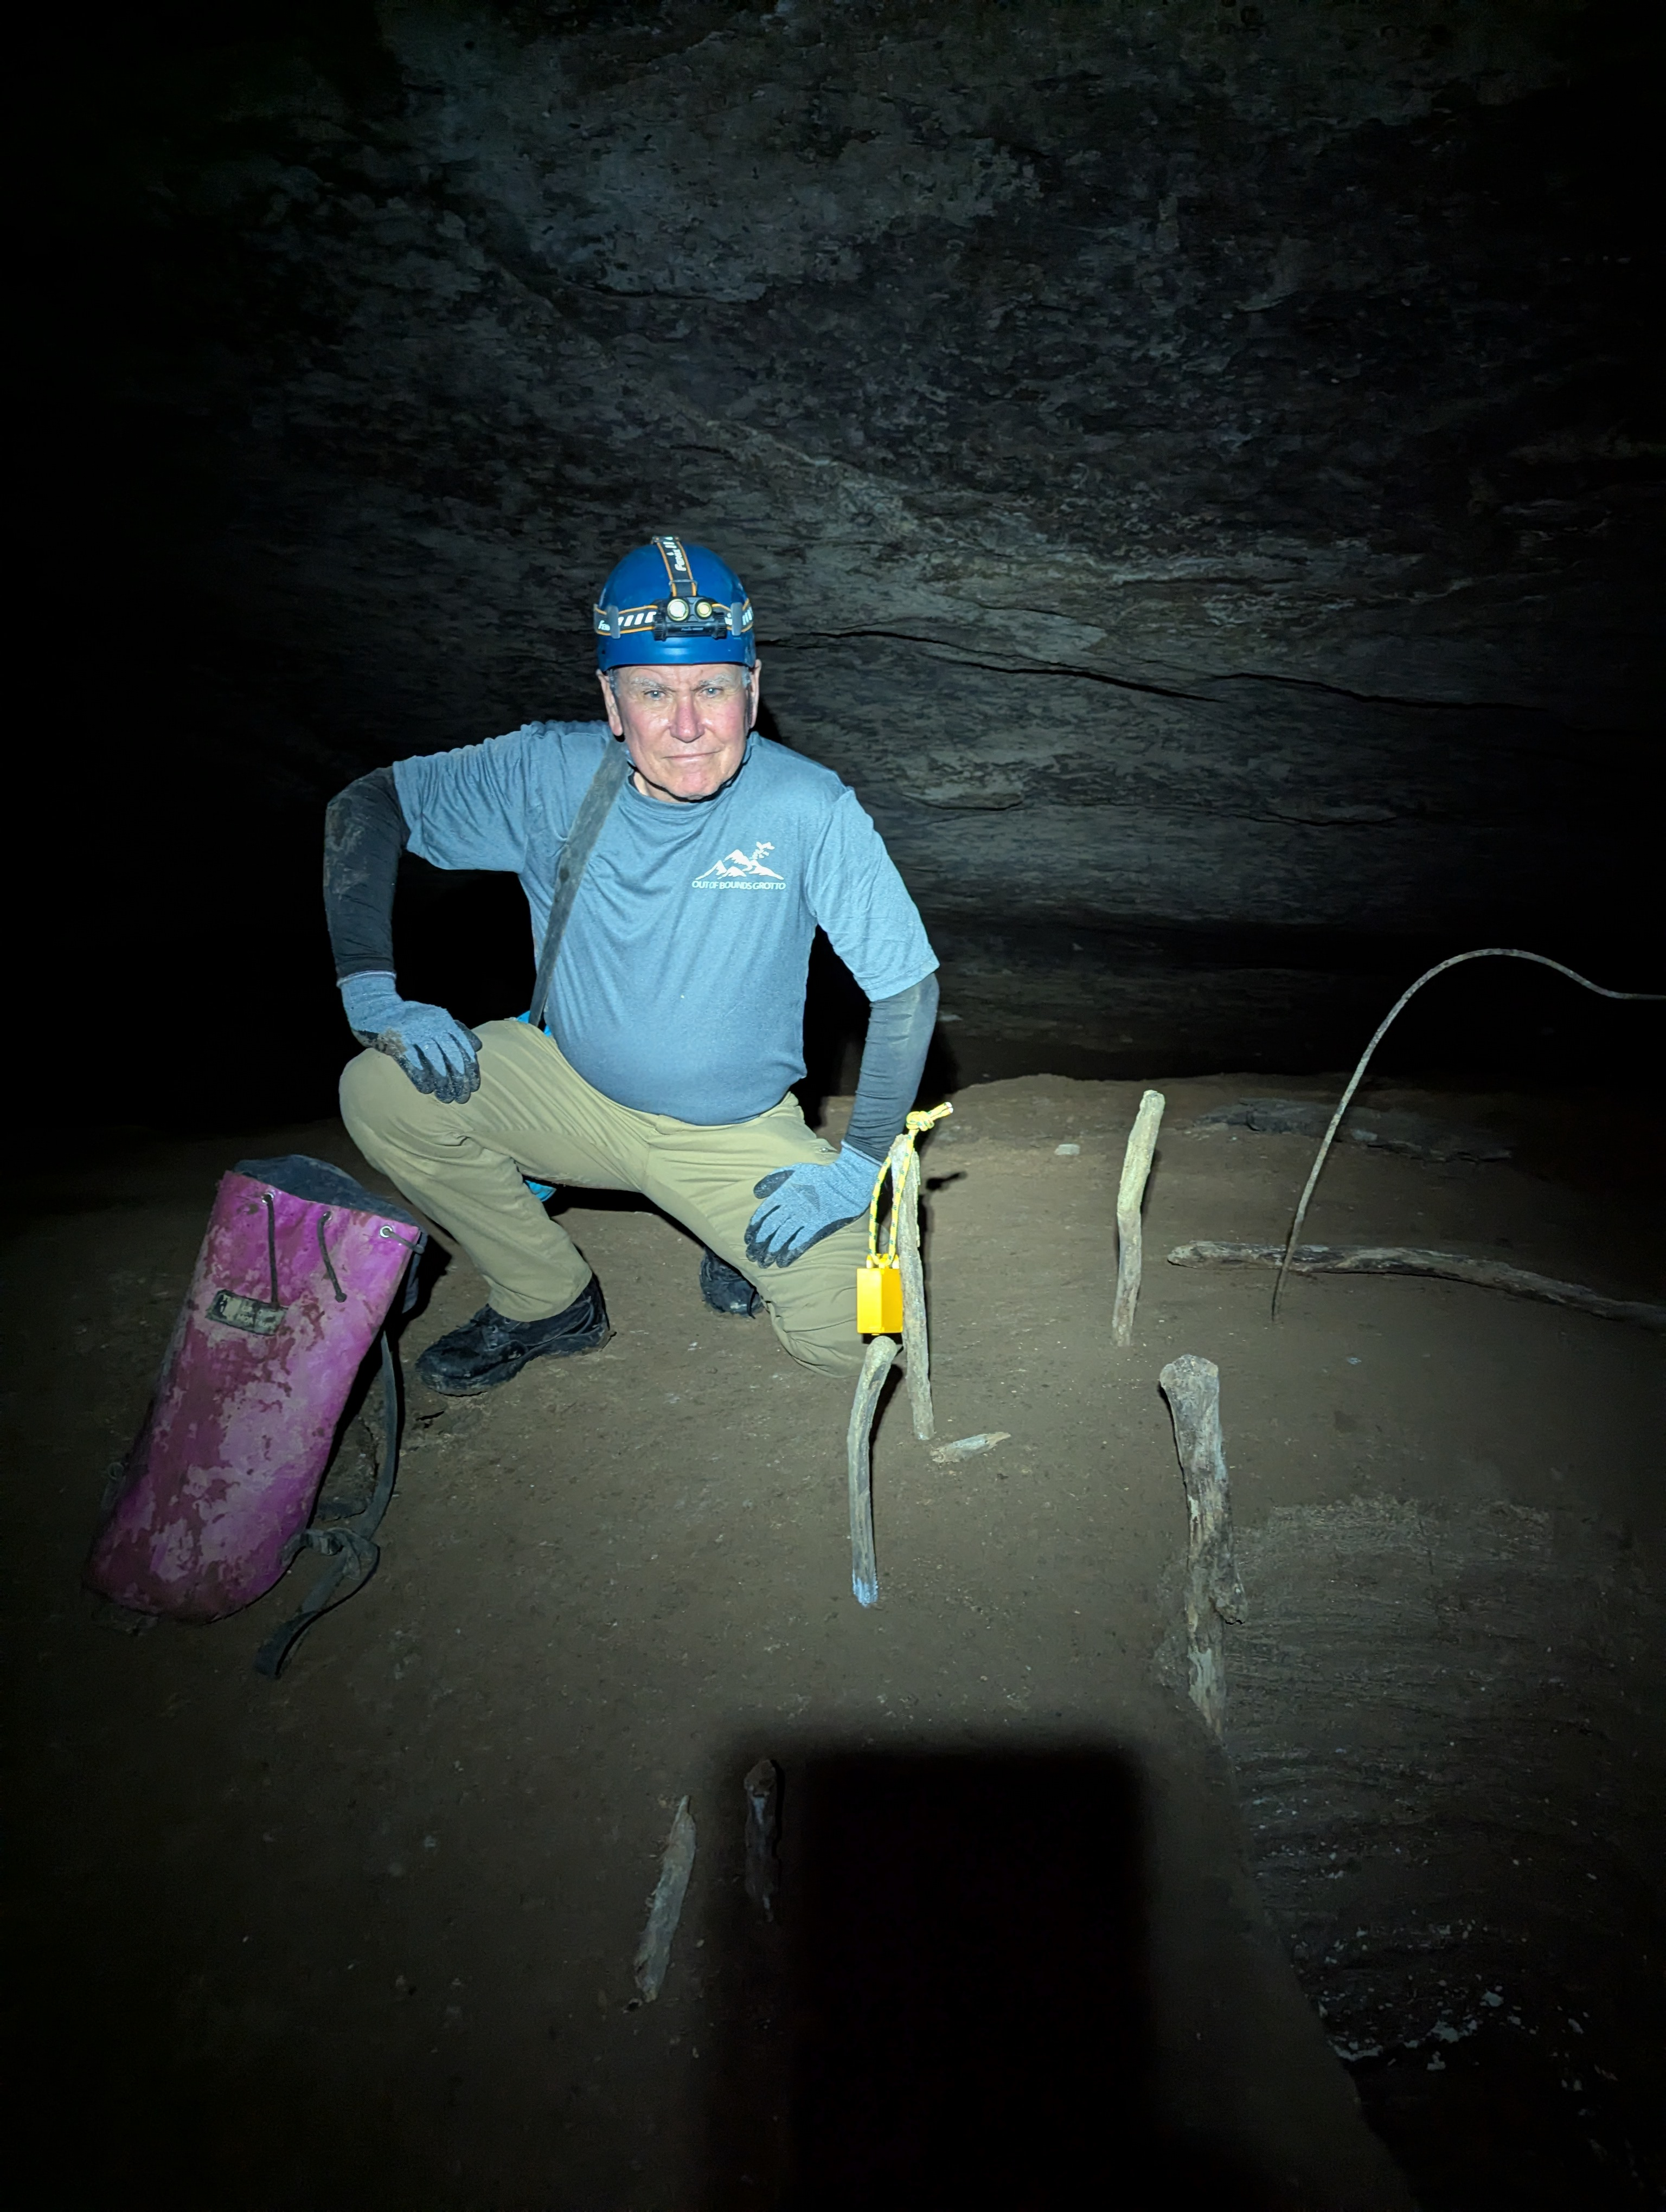
\includegraphics[width=.47\textwidth]{../images/PXL_20250610_223342846.jpg}
\end{center}

\end{frame}

\begin{frame}
\frametitle{Even More Nodes In Cave}

\begin{center}
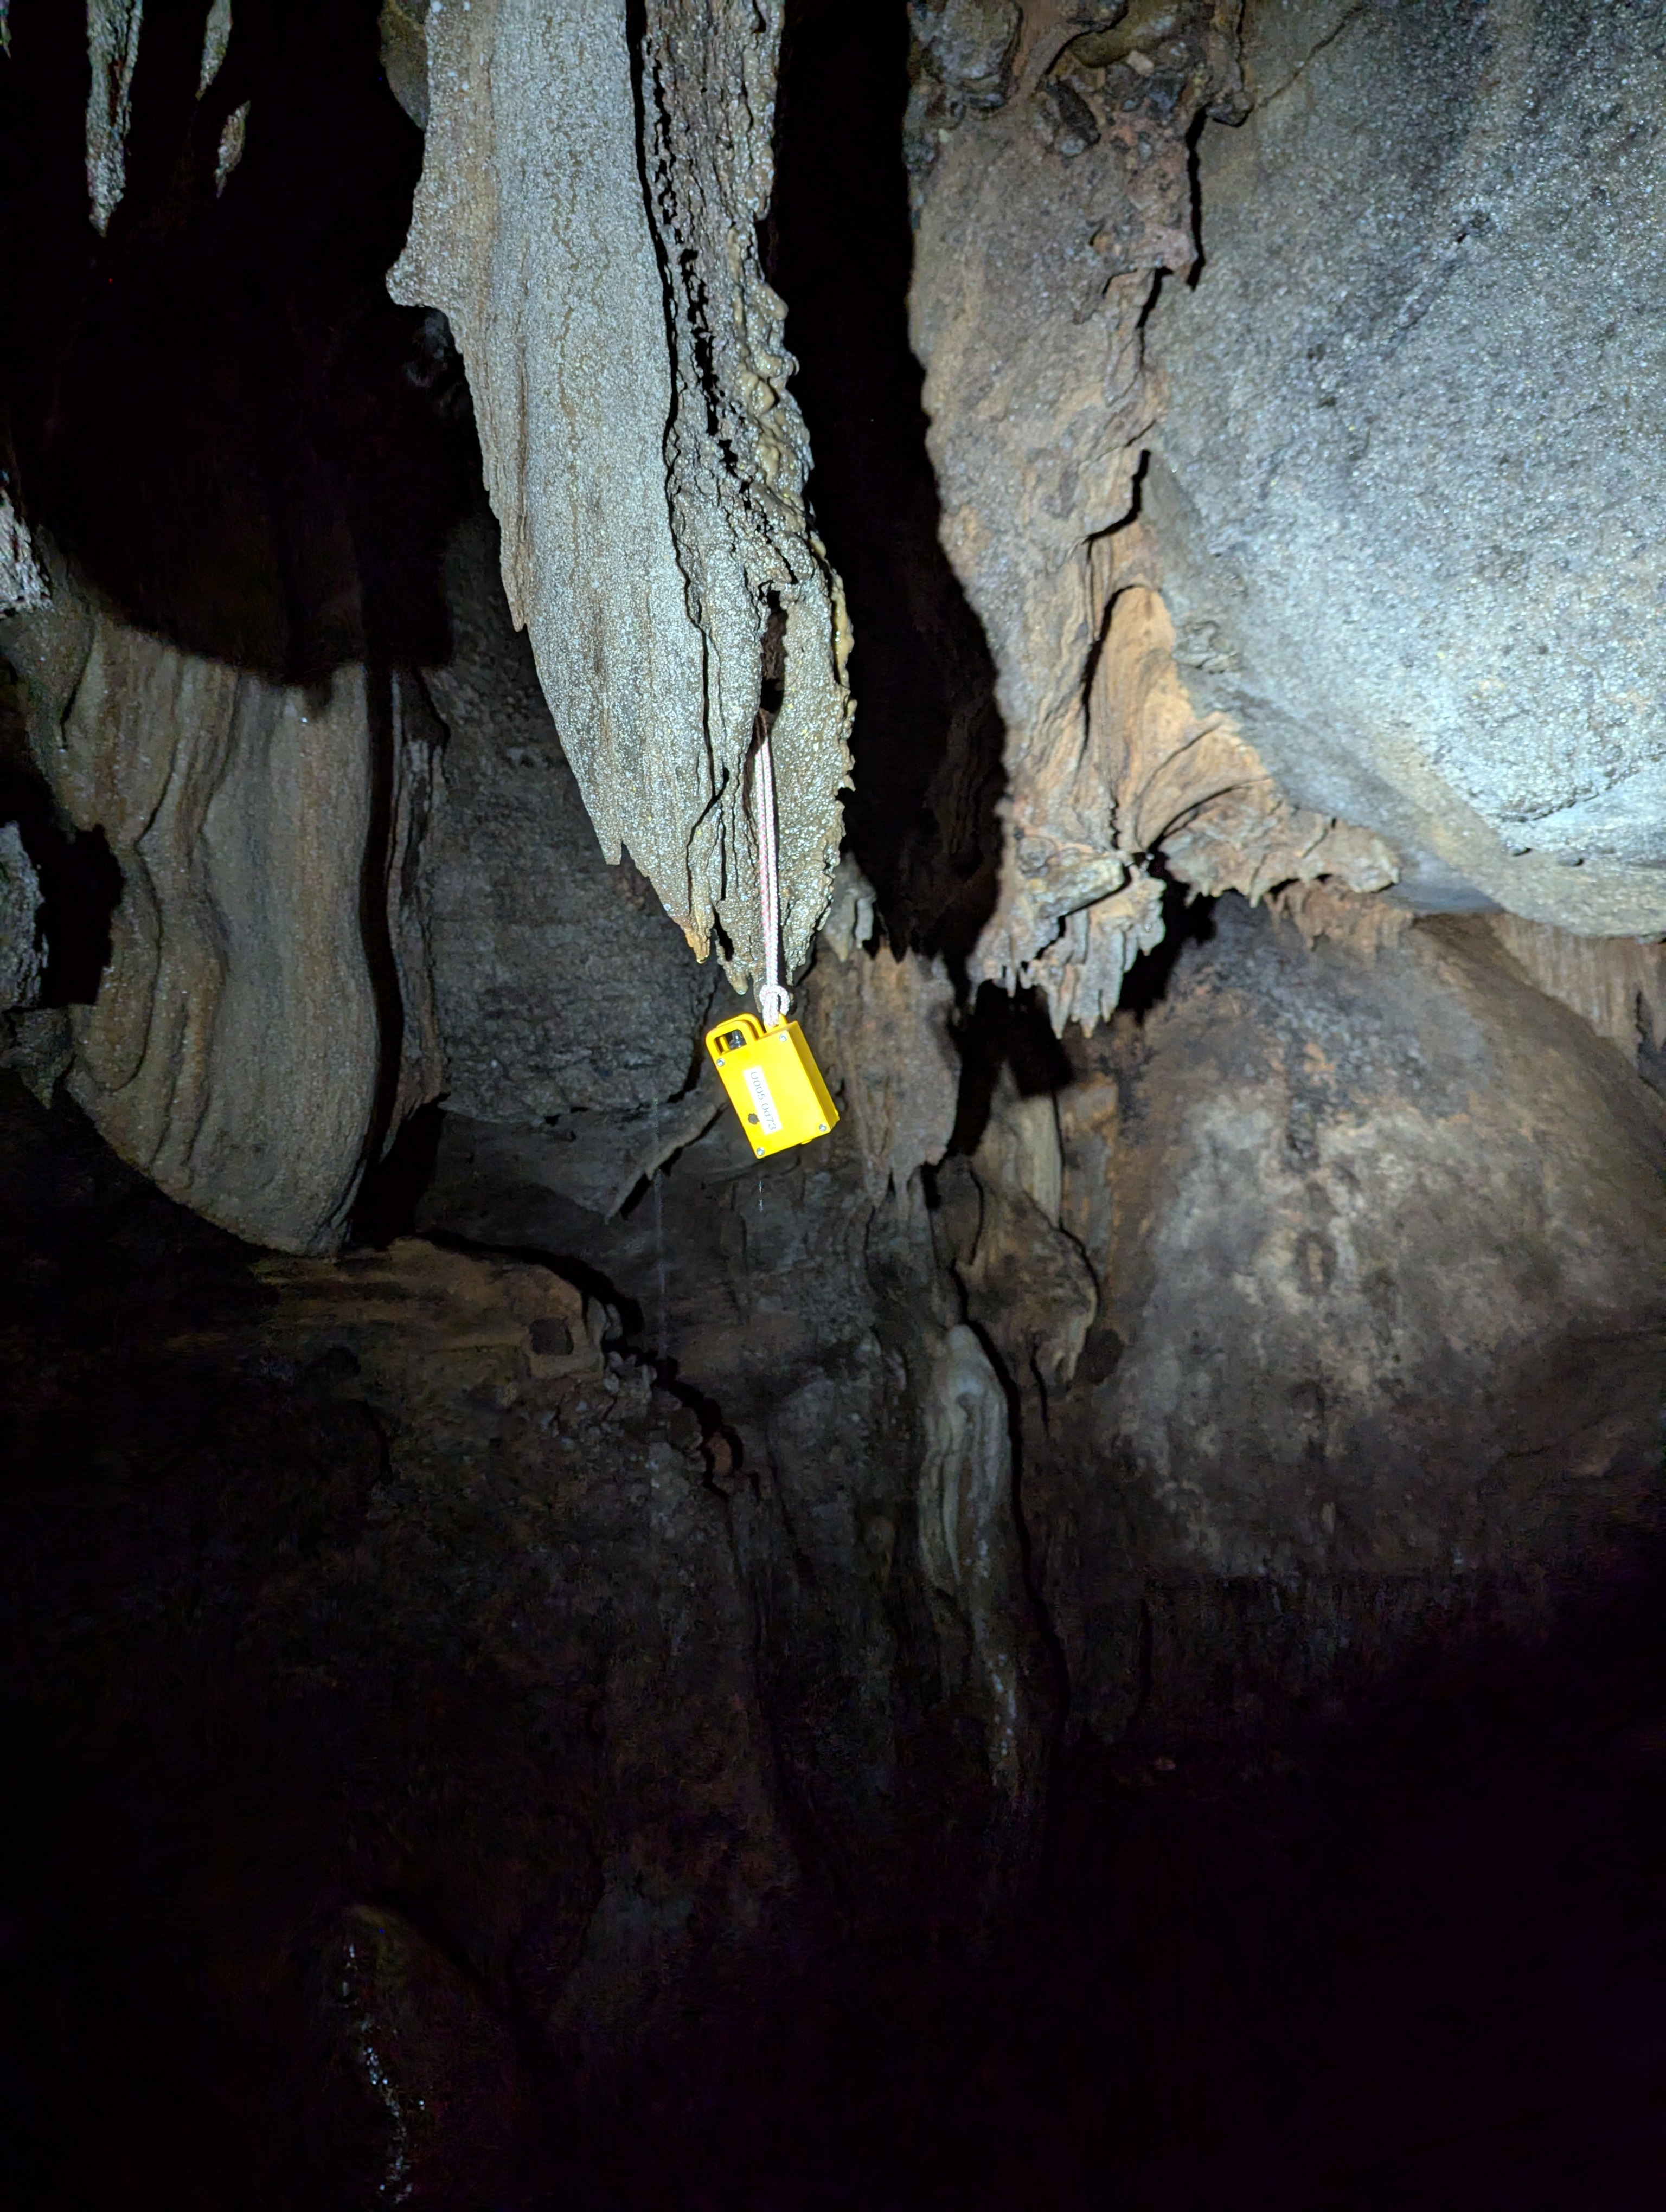
\includegraphics[width=.47\textwidth]{../images/PXL_20250610_231822265.LONG_EXPOSURE-01.COVER.jpg}\hfill
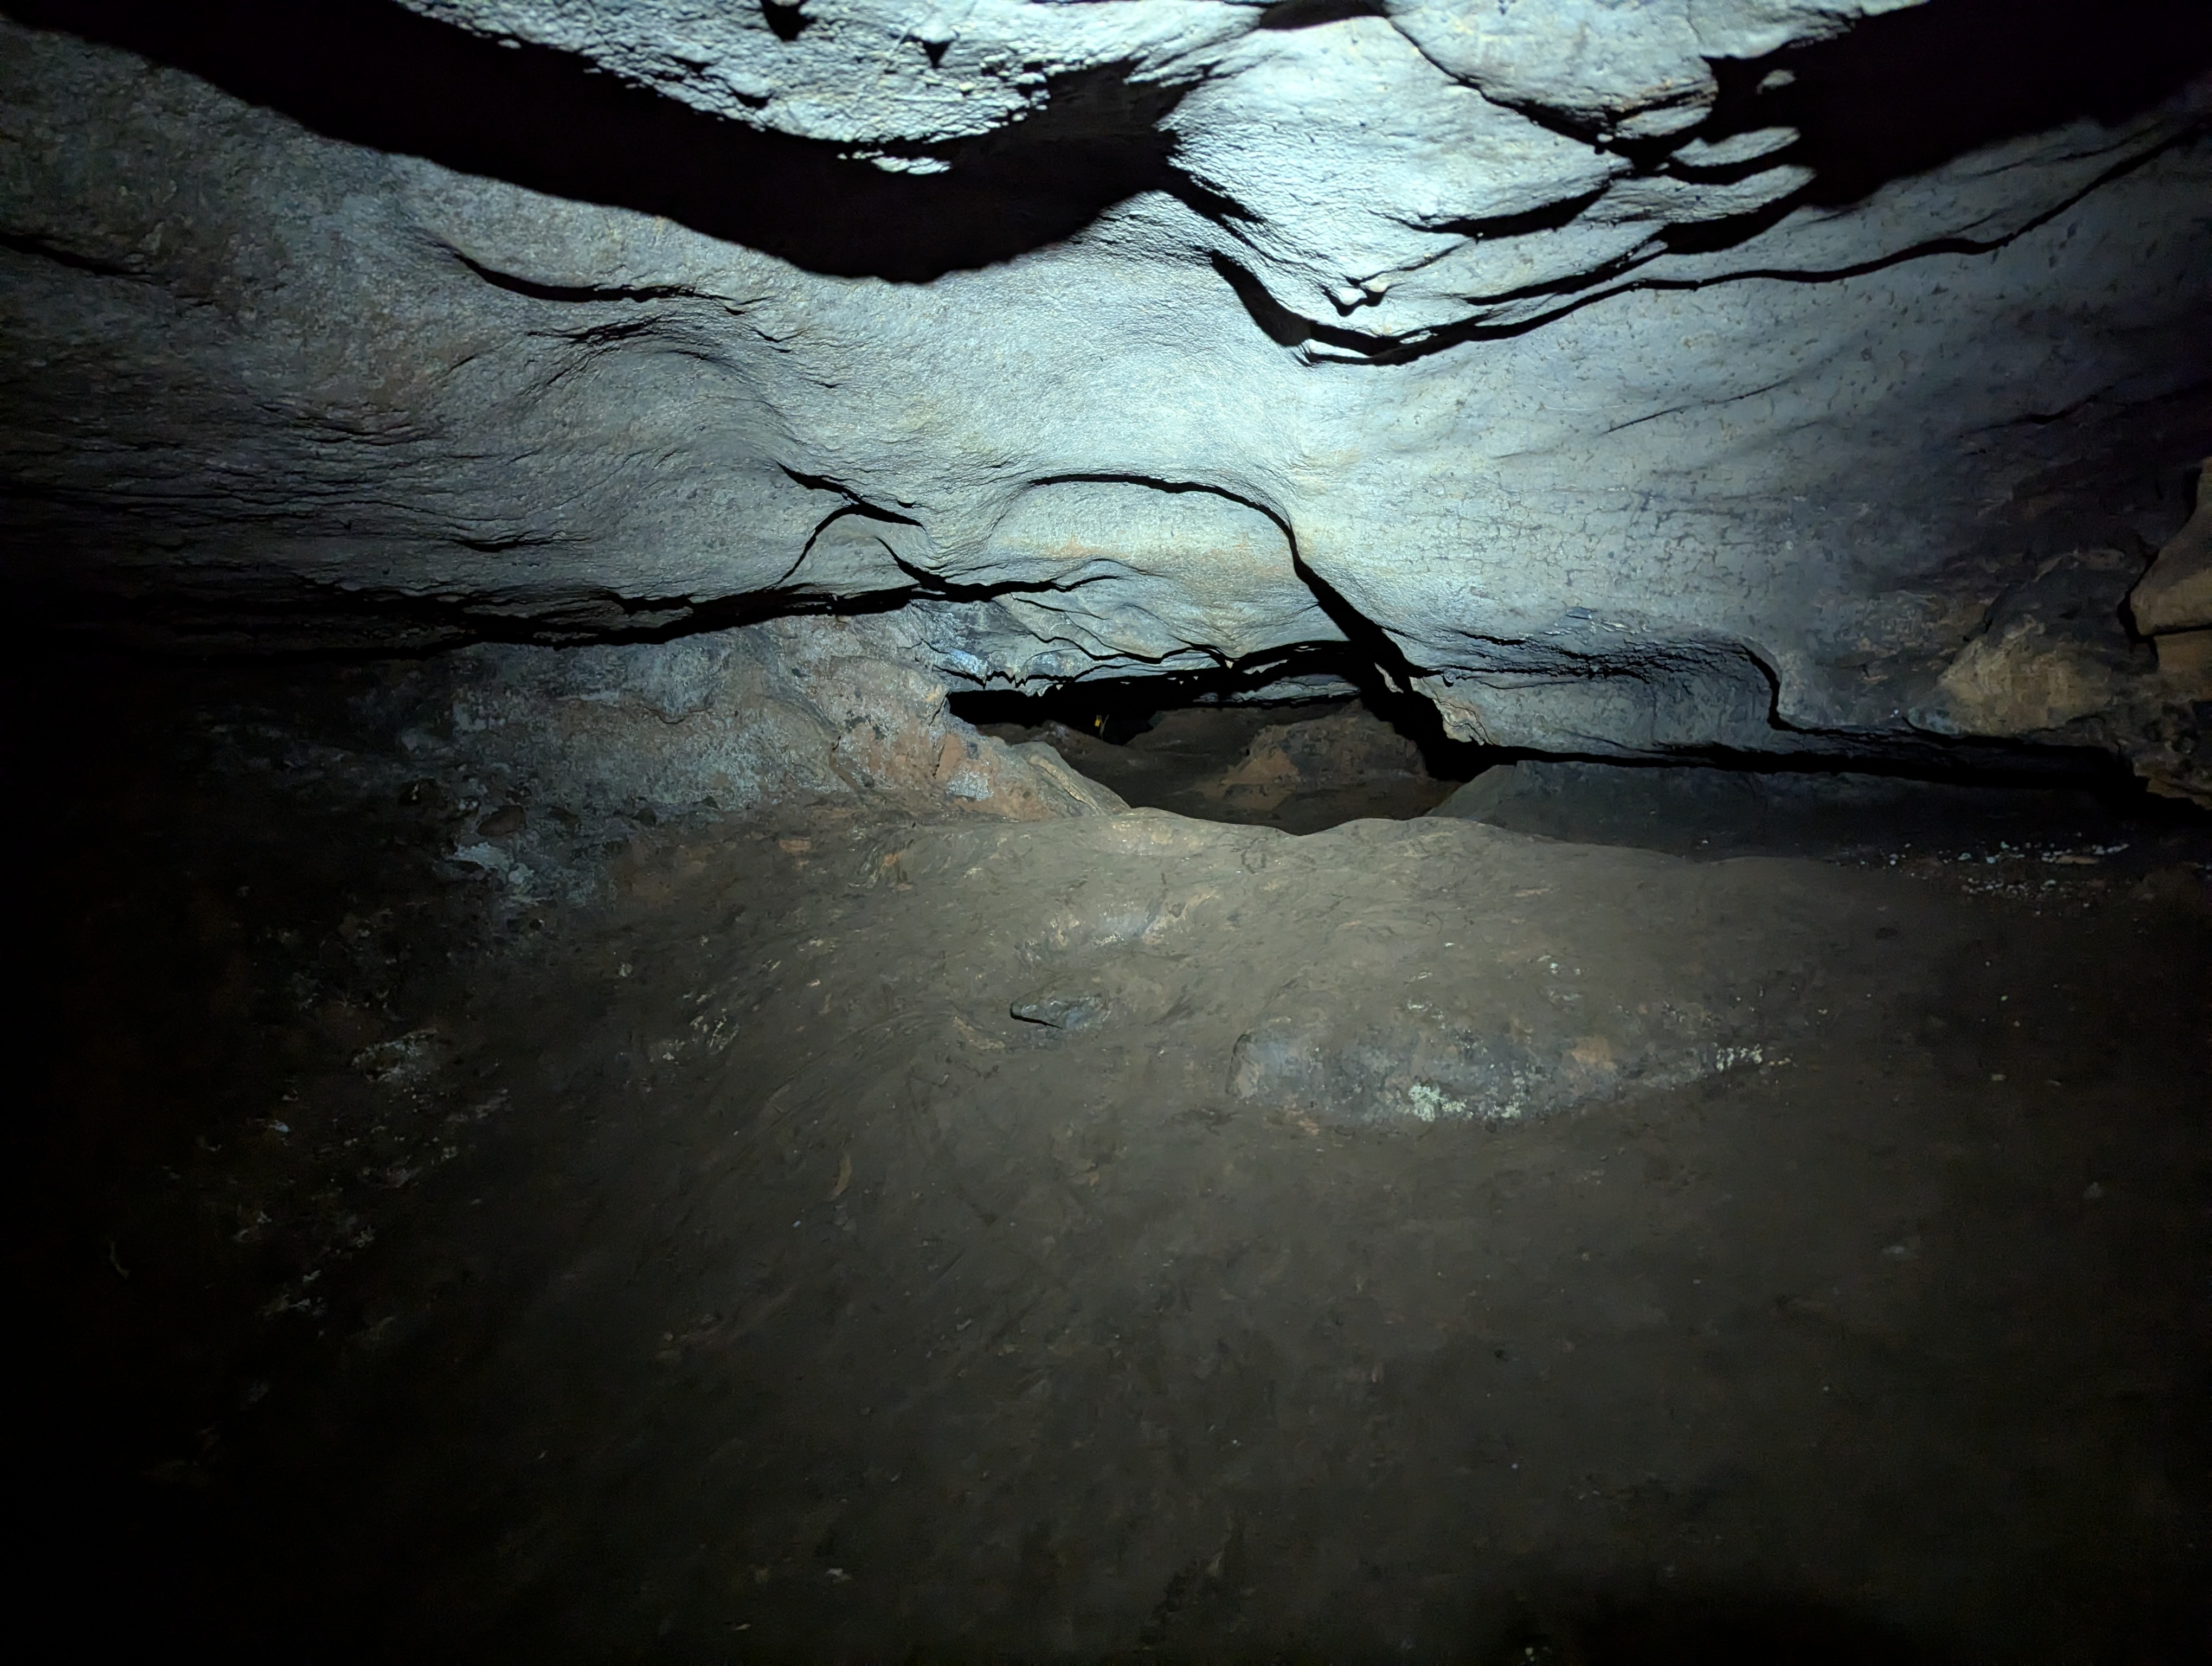
\includegraphics[width=.47\textwidth]{../images/PXL_20250610_231836339.LONG_EXPOSURE.jpg}
\end{center}

\end{frame}

\begin{frame}
\frametitle{Node Placement}

\begin{center}
\includegraphics[width=4.0in]{../images/Pig Hole Cave-10Jun25-mesh.png}
156m, 46m, 112m
\end{center}

\end{frame}

\section{Results}

\begin{frame}

\frametitle{Observations}

\begin{itemize}
\item We can communicate slightly past line of sight
\item Interoperating with surface meshs and mqtt is critical
\item Use lots of nodes to avoid premature optimization
\item Practice is critical
\item Communicators should carry a node
\item Automated ping bot is very useful for link testing
\end{itemize}

\end{frame}

\section{Where next?}

\begin{frame}
\frametitle{Future Work}

\begin{itemize}
\item Add point to point over wire capability
\item Test larger (10+) setups
\item Develop network mapping and traceroute tools
\item Collect all logs from nodes and analyze
\item More field tests, test in an actual mock rescue
\end{itemize}

\end{frame}

\begin{frame}
\frametitle{Related things}

\begin{itemize}
\item We deployed meshtastic nodes around campus with CO2 monitors
\item Huntsville video \tiny\url{https://www.youtube.com/watch?v=4BVUCpGBc3U}
\end{itemize}

\end{frame}

\begin{frame}
\frametitle{Conclusions}

\begin{itemize}
\item Technology looks good
\item Some development required
\item Using existing technology prevent reinventing a lot of wheels
\item Operator training critical (true for all comms)
\end{itemize}
\end{frame}

\begin{frame}
\frametitle{Questions}

Answer my Questions!

\end{frame}

\begin{frame}
\frametitle{Thanks}

\begin{itemize}
\item Steve Lepera - New case design
\end{itemize}

\end{frame}

\end{document}
